\section{Theory}\label{sec:Theory}

\newcommand{\state}{\ket{\psi}}
\newcommand{\hoket}{\ket{\phi}}
\newcommand{\hoep}{\ket{\phi +}}
\newcommand{\hoem}{\ket{\phi -}}
\newcommand{\pin}{\psi_\text{in}}
\newcommand{\pout}{\psi_\text{out}}
\newcommand{\kpin}{\ket{\psi_\text{in}}}
\newcommand{\kpout}{\ket{\psi_\text{out}}}
\newcommand{\mop}{\Omega_{+}}
\newcommand{\mom}{\Omega_{-}}
\newcommand{\melt}[3]{\left|\mel{#1}{#2}{#3}\right|^{2}}
\newcommand{\scat}{\mathcal{S}}
\newcommand{\mscat}{\(\scat\)}
\newcommand{\oop}[1]{\mathcal{#1}}
\newcommand{\moop}[1]{\(\oop{#1}\)}
Quantum scattering is a very complicated process, behaving so differently from the
classical case of billiard balls that our intuition breaks down. Fortunately, the intricacies of
the scattering process itself can be conveniently omitted by instead focusing on
the relationship between the initial and resulting states, illustrated in FIGURE.
Specifically, the true state \(\ket{\psi}\) is related to the asymptotic
incoming and outgoing states \(\kpin\) and \(\kpout\) through the so-called
\textit{M\o ller operators} \(\Omega_{\pm}\):

\begin{align*}
  \state &= \mop\kpin = \hoep\\
  \state &= \mom\kpout = \hoem .
\end{align*}
[Add some history of Møller]

If time dependence is added, the M\o{}ller operations allows one to move between
the asymptotic states and the actual state at time \(t\).
Combining them, the outgoing state is related to the incoming state by

\begin{equation*}
  \kpout = \mom^{\dagger}\mop\kpin = \scat\kpin
\end{equation*}

giving the definition of the \textit{scattering operator} \mscat.
In the general case, let \(\ket{\chi -}\) and \(\ket{\Phi +}\) be any arbitrary
orbits. The probability of the process \(\ket{\Phi +}\to\ket{\chi -}\)
occurring is
then the square of the  matrix element of\ \mscat :

\begin{equation*}
  w(\chi \leftarrow \Phi) = \left| \ip{\chi -}{\Phi +} \right|^{2} = \melt{\chi}{\scat}{\Phi}.
\end{equation*}

While the probability \(w\) itself is not observable, the related quantity
cross-section \mbox{\(\sigma(\chi \leftarrow \Phi)\)} is. The outgoing particle can
scatter into a solid angle \(d\Omega\), oriented in the direction of momentum
\(\vec{p}\). Likewise, the incoming particle can be described as wave packets
with narrowly defined momentum \(\vec{p_{0}}\). It can then be
shown\cite[p.~51]{taylor} that the
differential cross section is

\begin{align*}
  \dv{\sigma}{\Omega}(\vec{p}\leftarrow\vec{p_{0}}) = \left| f(\vec{p}\leftarrow\vec{p_{0}}) \right|^{2}
\end{align*}
with \(f(\vec{p}\leftarrow \vec{p_{0}})\) being the scattering amplitude, as known from elementary scattering
theory. Note that only the magnitude of \(f\) can be obtained through the
cross-section.

The next step is to relate cross-section to the scattering operator. It
can be shown\cite[p.~40] that \mscat{} commutes with the free Hamiltonian \( \oop{H}_{0}\)
\begin{align*}
  \oop{H} = \oop{H}_{0} + V &\qquad [\oop{H}_{0}, \scat{}] = 0
\end{align*}
Letting \(\ket{\vb{p}}\) be the eigenvectors of \(\oop{H}_{0}\) in momentum
basis, we have
\begin{align*}
  \mel{\vb{p}^{\prime}}{[\oop{H}_{0}, \scat]}{\vb{p}} = (E_{p^{\prime}}-E_{p})\mel{\vb{p}^{\prime}}{\scat}{\vb{p}} = 0
\end{align*}
implying that \(\mel{\vb{p}^{\prime}}{\scat}{\vb{p}}\) is zero except for
\(E_{p^{\prime}}=E_{p}\). This leads to the form
\begin{align*}
  \mel{\vb{p}^{\prime}}{\scat}{\vb{p}} = \delta(E_{p^{\prime}}-E_{p})\times\text{remainder}
\end{align*}

At this point it is fruitful to define a new operator \(\oop{R} \equiv 1 -
\scat\). \moop{R} is the difference between the case of scattering and no scattering. It too commutes with \(\oop{H}_{0}\), and so has the form
\begin{align*}
  \mel{\vb{p}^{\prime}}{\oop{R}}{\vb{p}} = -2\pi i\delta(E_{p^{\prime}}-E_{p})t(\vb{p}^{\prime}\leftarrow \vb{p})
\end{align*}
with the factors \(-2\pi i\) and \(t(\vb{p}^{\prime}\leftarrow\vb{p})\)
introduced for future convenience. The elements of\ \mscat{} can therefore be written 
\begin{align*}
  \mel{\vb{p}^{\prime}}{\scat}{\vb{p}} = \delta(\vb{p}^{\prime} - \vb{p}) - 2\pi i \delta(E_{p^{\prime}}-E_{p})t(\vb{p}^{\prime}\leftarrow \vb{p}).
\end{align*}
 The function
\(t(\vb{p}^{\prime}\leftarrow \vb{p})\) is continuous for most potentials and
analytic for many, but only defined for the ``shell'' \(\vb{p}^{{\prime}^{2}} =
\vb{p}^{2}\). However unphysical, it is computationally beneficial to define an
operator \moop{T} whose matrix elements \(\mel{\vb{p}^{\prime}}{T}{\vb{p}}\) are defined for all \(\vb{p}\) and
coincide with the values of \(t\) on the shell.

The scattering amplitude can be shown to be related to the on-shell \moop{T}
matrix elements as\cite[p.~172]{taylor}
\begin{align*}
  f(\vb{p}^{\prime} \leftarrow \vb{p})= -(2\pi)^{2}mt(\vb{p}^{\prime}\leftarrow\vb{p}).
\end{align*}
The elements of the scattering matrix can thus be written in terms of the
scattering amplitude:
\begin{align*}
  \mel{\vb{p}^{\prime}}{\scat}{\vb{p}} = \delta(\vb{p}^{\prime} - \vb{p}) - \frac{i}{2\pi m}\delta(E_{p^{\prime}}-E_{p})f(\vb{p}^{\prime}\leftarrow \vb{p}).
\end{align*}
The first term describes the situation where no scattering occurs, while the
second is the amplitude for when the wave is actually scattered, with the
probability being the square of the scattering amplitude, hence its name.
\subsection{Spherical Coordinates}

Introducti

As known from elementary quantum mechanics, \(\oop{H}^{0}\) commutes with the
angular momentum operator \(\oop{L}^{2}\) and z-axis projection \(\oop{L}_{3}\).
These three operators form a complete set of commuting observables. As 
\mscat{} commutes with \(\oop{H}^{0}\), \mscat{} too commutes with the
aforementioned 
operators, and is diagonal in the common basis, namely the basis of spherical waves
\(\left\{ \ket{Elm} \right\}\), with \(E, l(l+1)\) and \(m\) being the
eigenvalues for \(\oop{H}^{0}\),  \(\oop{L}^{2}\) and  \(\oop{L}_{3}\)
respectively. Since this basis diagonalizes\ \mscat{}, its matrix elements in
this basis are
\begin{align*}
  \mel{E^{\prime}l^{\prime}m^{\prime}}{\scat}{Elm} = \delta(E^{\prime}-E)\delta_{l^{\prime}l}\delta_{m^{\prime}m}s_{l}(E).
\end{align*}

\mscat{} can be shown to be unitary, implying the eigenvalues \(s_{l}(E)\) must have
modulus one, justifying the form
\begin{align*}
  \mel{E^{\prime}l^{\prime}m^{\prime}}{\scat}{Elm} = \delta(E^{\prime}-E)\delta_{l^{\prime}l}\delta_{m^{\prime}m}\exp(2i\delta_{l}(E))
\end{align*}
The quantity \(\delta_{l}(E)\) is the important \textit{phase shift}, an
observable obtainable from both experiment and numerical calculations. It is
purely real with an inherent ambiguity modulo \(\pi\), as seen from
\begin{align*}
  \exp(2i[\delta_{l}+n\pi]) = \exp(2i\delta_{l})\exp(2in\pi) = \exp(2i\delta_{l}).
\end{align*}

[Meaning of T in the sense incident plane wave]
[]

The decomposition of \(f(\vb{p}^{\prime}\leftarrow\vb{p})\) into partial waves
can be obtained by exploiting the relation

\begin{equation}
  \label{eq:sp1}
  \mel{\vb{p}^{\prime}}{(\scat-1)}{\vb{p}} = \frac{i}{2\pi m}\delta(E^{\prime}-E)f(\vb{p}^{\prime}\leftarrow \vb{p}).
\end{equation}
Inserting a complete set of states of the left hand side gives
\begin{align*}
  \mel{\vb{p}^{\prime}}{(\scat-1)}{\vb{p}} &= \int \dd E \sum_{l, m}  \mel{\vb{p}^{\prime}}{(\scat-1)}{Elm}\ip{Elm}{\vb{p}}\\
                                             &=  \int \dd E \sum_{l, m} (s_{l}(E)-1) \ip{\vb{p}^{\prime}}{Elm}\ip{Elm}{\vb{p}}\\
  &= \frac{1}{mp}\delta(E_{p^{\prime}}-E_{p})\sum_{l,m}Y_{l}^{m}(\vu{p}^{\prime})[s_{l}(E_{p})-1]Y^{m}_{l}(\vu{p})^{*}
\end{align*}
where \(Y_{l}^{m}\) are the spherical harmonicals and the \(\hat{\text{hat}}\) denotes unit vector. Combining this
with~\eqref{eq:sp1}, the amplitude can be decomposed to

\begin{align*}
  f(\vb{p}^{\prime}\leftarrow\vb{p}) = \frac{2\pi}{ip}\sum_{l,m}Y_{l}^{m}(\vu{p}^{\prime})[s_{l}(E_{p})-1]Y^{m}_{l}(\vu{p})^{*}
\end{align*}
Letting \(\vu{p}\) lie along \(z\) and noting independence of \(m\) [WHY], we
define
\begin{align*}
  f(E_{p},\theta) \equiv f(\vb{p}^{\prime}\leftarrow\vb{p})=\frac{1}{2ip}\sum_{l}(2l+1)[s_{l}(E_{p})-1]P_{l}(\cos\theta)
\end{align*}
This leads to the natural definition of the \textit{partial wave amplitude} as
\begin{align*}
  f_{l}(E) \equiv \frac{s_{l}(E)-1}{2ip} = \frac{\exp[ 2i\delta_{l}(\theta)] - 1}{2ip} = \frac{\exp[2i\delta_{l}(E)]\sin\delta_{l}(E)}{p}
\end{align*}
Analogously the total cross-section can be decomposed into \textit{partial wave
  cross-sections}, giving
\begin{align*}
  \sigma(p) = \sum_{l}\sigma_{l}(p) = \sum_{l}4\pi(2l+1)\left| f_{l}(p) \right|^{2} = \sum_{l}4\pi(2l+1)\frac{\sin^{2}\delta_{l}}{p^{2}}
\end{align*}
The magnitude of each partial wave cross-section is from this constrained by the
so called \textit{unitary bound}: 
\begin{align*}
  |\sigma_{l}| \leq 4\pi\frac{2l+1}{p^{2}}.
\end{align*}
The maximal value is only reached if
\(\delta_{l}\) is an odd multiple of \(\pi/2\)

General properties of the scattering process can be found by studying both the
general and the limiting forms of the wave function. As before, the wave
function of the full Hamiltonian
\(\ip{vb{x}}{Elm+}\) can be obtained from the wave function of the free Hamiltonian by the Møller operator
\begin{equation*}
  \ip{\vb{x}}{Elm+} = \Omega_{+}\ip{\vb{x}}{Elm},
\end{equation*}
and hence we can get away with studying the free wave. From basic quantum
mechanics, we know it is on the form
\(\frac{1}{r}y(r)Y^{m}_{l}(\vu{x})\) with \(y(r)\) satisfying the radial
Schr\"odinger equation

\begin{equation*}
  \left[ \dv[2]{r} - \frac{l(l+1)}{r^{2}}+p^{2}\right]y(r) = 0.
\end{equation*}
\newcommand{\rbf}{\hat{j}_l(z)}
When \(r\to 0\), \(y(r)\) must go as\(r^{-l}\) or \(r^{l+1}\). The latter
condition is satisfied by the
Riccati-Bessel functions \(\rbf{} = zj_{l}(z)\). Its limiting behavior as \(z\to
0\) is
\begin{equation*}
  \rbf{} \xlongrightarrow[z\to 0]{} \frac{z^{l+1}}{(2l+1)!!}\left[ 1+\mathcal{O}(z^{2}) \right]
\end{equation*}
The other limiting condition is satisfied by the Riccati-Neumann function
\(\hat{n}_{l}(z)\). 

Hence
\begin{equation}
  \label{eq:xelm}
  \ip{\vb{x}}{Elm} = i^{l}\left( \frac{2m}{\pi p} \right)^{1/2}\frac{1}{r}\hat{j}^{l}(pr)Y^{m}_{l}(\vu{x})
\end{equation}

On the other side, the limit \(r\to\infty\) requires the boundary conditions
\(e^{\pm ipr}\). These are satisfied by the Riccati-Hankel functions
\(\hat{h}_{l}^{\pm}(z) = \hat{n}_{l}(z) \pm ij_{l}(z)\). Its limiting form is
\begin{equation*}
  \hat{h}^{\pm}_{l}(z) = e^{\pm i\left( z-l\pi/2 \right)}\left[ 1+\mathcal{O}(z^{-1}) \right]
\end{equation*}

In analogy to~\eqref{eq:xelm}, the full wave function can be written as
\begin{equation*}
  \ip{\vb{x}}{Elm+} = i^{l}\left( \frac{2m}{\pi p} \right)^{1/2}\frac{1}{r}\psi_{lp}(r)Y^{m}_{l}(\vu{x})
\end{equation*}
from which we see that \(\psi_{lp}(r)\to\hat{j}_{l}(pr)\) when \(V\to 0\). In
the other limiting case \(r\to \infty\), it can be shown~\cite[p.~187]{taylor} to be
\begin{equation*}
  \psi_{lp}(r)   \xlongrightarrow[r\to \infty]{} \hat{j}_{l}(pr)+pf_{l}\hat{h}^{+}_{l}(pr).
\end{equation*}
Using the limiting forms of the functions and some algebra, this can be
rewritten as
\begin{equation*}
  \psi_{lp}(r)   \xlongrightarrow[r\to \infty]{} e^{i\delta_{l}(p)}\sin\left[ pr - \frac{1}{2}l\pi+\delta_{l}(p) \right]
\end{equation*}
This makes significance of the phase shift apparent. At large \(r\) the actual
wave function becomes proportional to the free wave function
\begin{equation*}
  \hat{j}_{l}(pr)\to\sin\left( pr-\frac{1}{2}l\pi \right)
\end{equation*}
except that its oscillations are shifted by the phase shift \(\delta_{l}\).


\subsection{Green's Function}
One of the most important tools in scattering theory is \textit{the resolvent},
or \textit{Green's operator}. For many types of integral equations, a Green's
function can be associated, transforming the solving of the equation to the
computation of the Green's function. For our purposes the most important Green's
operators are the \textit{free Green's operator}

\begin{equation*}
  \oop{G}^{0}(z) \equiv (z-\oop{H}^{0})^{-1}
\end{equation*}
and the \textit{full Green's operator}
\begin{equation*}
  \oop{G}(z) \equiv (z-\oop{H})^{-1}
\end{equation*}
with \(z\in\mathbb{C}\). Without loss of generality, assume the spectrum of
\(\oop{H}\) is discrete, with the orthonormal basis \({\ket{n}}\). Then the full
Green's operator can be written

\begin{equation*}
  \oop{G}(z) = (z-\oop{H})^{-1}1 = \sum_{n}\frac{\op{n}}{z-E_{n}}.
\end{equation*}
A specific matrix element is therefore
\begin{equation*}
  \mel{\chi}{\oop{G}(z)}{\psi} =\sum_{n} \frac{\ip{\chi}{n}\ip{n}{\psi}}{z-E_{n}}.
\end{equation*}
\newcommand{\gop}{\oop{G}(z)}
\newcommand{\mgop}{\(\oop{G}(z)\)}
For any \(z\) not an eigenvalue \(E_{n}\), the matrix element is well defined and
analytic. When \(z\) is an eigenvalue, it is a simple pole with residue
\(\ip{\chi}{n}\ip{n}{\psi}\). That is, knowing the poles of \(\oop{G}(z)\) gives
information about the corresponding eigenvectors. As both the energy
eigenvectors and eigenvalues can be found from \mgop{} itself, knowledge of
\mgop{} is equivalent to solving the eigenvalue problem of
\(\oop{H}\)\footnote{Of course, this is merely an intuitive explanation, not a
  proof. It can be shown that this is indeed true in the general case, see~\cite[p.~131]{taylor}}

While discrete spectra lead to poles in \(\mel{\chi}{\gop{}}{\psi}\), continuous spectra lead to 
branch cuts. Consider the free Green's operator, which in terms of the angular
momentum eigenvectors in analogy to the discrete spectrum has the matrix elements

\begin{equation*}
  \mel{\chi}{\oop{G}^{0}(z)}{\psi} = \int_{0}^{\infty}\frac{\dd E}{z-E}\left\{
  \sum_{l,m}\ip{\chi}{Elm}\ip{Elm}{\psi}
  \right\}
\end{equation*}

that again gives well-defined functions for \(z\notin\mathbb{R}^{+}\). For any
\(E^{0} > 0\), the integral diverges. This can be seen by taking the difference
between approaching the axis from the top and approaching it from the bottom,
yielding\cite[p.~469]{messiah} \(2\pi i \sum_{lm}\op{Elm}\).

The scattering process can yield both scattered states and bound states. The
former is associated with continuous spectra while the latter with discrete.
From the discussion above, scattered states correspond with branch cuts
along \(E^{0}>0\) while bound states show up as simple poles in \(\oop{G}(z)\).

Finding \(\oop{G}(z)\) is just as difficult as solving the eigenvalue problem
for \(\oop{H}\). Using \(\oop{G}(z)\), however, yields an alternative numerical
approach while at the same providing a powerful theoretical tool. The first step
is to write \(\oop{G}(z)\) in terms of the simpler \(\oop{G}^{0}(z)\). This is
trivially done using the algebraic relation

\begin{equation*}
  \oop{A}^{-1} = \oop{B}^{-1} + \oop{B}^{-1}(\oop{B}-\oop{A})\oop{A}^{-1}.
\end{equation*}
Inserting \(\oop{A} = z-\oop{H}\) and \(\oop{B} = z-\oop{H}^{0}\) gives
\begin{equation}
  \label{eq:LSG}
  \gop = \gop{}^{0} + \gop{}^{0}V\gop{} = \gop{}^{0} + \gop{}V\gop{}^{0}.
\end{equation}
This is known as the \textit{Lippmann-Schwinger equation for \mgop{}}.


\subsection{Lippman Schwinger}

The Lippmann-Schwinger equation turns out to be a common and useful relation
between operators in scattering theory. The derivation through Green's operators
is not the historic path, and has the downside of obscuring its physical
relationship to the Schr\"odinger equation.

[intro]
Out of thin air we define the operator \(\oop{T}\) as the potential plus the
distortion to the potential caused by the full Green's operator:

\begin{equation}
  \label{eq:T}
  \oop{T}(z) = V + V\oop{G}V.
\end{equation}
It is clear that \(\oop{T}(z)\) has the same properties as \mgop{} with respect
to poles and branch cuts. Combining~\eqref{eq:T} with~\eqref{eq:LSG} together
with some algebraic manipulations, we obtain the Lippmann-Schwinger equation for \(\oop{T}(z)\):

\begin{equation}
  \label{eq:LST}
 \oop{T}(z) = V + V\oop{G}^{0}(z)\oop{T}(z).
\end{equation}

In momentum space~\eqref{eq:LST} is written as

\begin{equation*}
  \mel{\vb{p}^{\prime}}{\oop{T}(z)}{\vb{p}} = \mel{\vb{p}^{\prime}}{V}{\vb{p}}
  + \int\dd^{3}p^{''} \frac{\mel{\vb{p}}{V}{\vb{p^{''}}}}{z-E_{p^{''}}}\mel{\vb{p}^{''}}{T(z)}{\vb{p}}
\end{equation*}

This highlights the need for introducing the \(\oop{T}\) operator in the first
place. There is no LS equation for the \(\oop{S}\) because it requires the
operators to be smooth functions, while \(\oop{S}(z)\) is
highly singular. On the other hand \(\oop{T}\) analytic almost everywhere,
allowing it to be expressed in terms of an integral equation. 

Through a long and rather limit-finicky derivation, the \moop{S} operator can be
derived in terms of the \moop{T} operator when \(z\) approaches the real axis
from above
\begin{equation*}
  \mel{\vb{p}\prime}{S}{\vb{p}} = \delta(\vb{p}^{\prime}-\vb{p}) -2\pi i\delta(E_{p^{\prime}}-E_{p})
  \lim_{\epsilon\downarrow 0}\mel{\vb{p}^{\prime}}{T(E_{p}+i\epsilon)}{\vb{p}}.
\end{equation*}
This relation being the main motivation for defining \moop{T} in the first
place. It shows that \(t(\vb{p}^{\prime}\leftarrow\vb{p})\) corresponds to the
on-shell \(T\)-matrix.

A reasonable question to ask is why computing the entire \(T\)-matrix is
necessary when only the on-shell elements are physical. As already mentioned,
one reason is computational; The on-shell elements are the limiting quantities
of the off-shell elements. This doesn't mean that the off-shell elements are
only a mathematical necessity. In fact, they correspond to the virtual
interactions in the scattering process, which accounts for their fundamental
unmeasurable nature. We are only allowed to observe the scattering in the
non-interacting region, being the limiting case of the unobservable processes
happening inside of the interacting region. Our initial starting point of
focusing on the asymptotic states while ignoring the intricacies of the
scattering is therefore not some mathematical trick to make computation easier,
but an unavoidable requirement.

\subsection{The K-Matrix}

The Lippmann-Schwinger equation for \(\oop{T}\) can not be solved by simple
analytical methods. One recourse is to use approximation techniques. These are
based on the expansion of \(\oop{T}\) into the 
infinite sum
\begin{equation*}
  \oop{T} = V + V \frac{1}{E-H^{0}+i\epsilon}V + V \frac{1}{E-H^{0}+i\epsilon}V \frac{1}{E-H^{0}+i\epsilon} V+\ldots
\end{equation*}
The unitarity condition of \(\oop{T}\) is satisfied for the whole series, but
violated for any finite order. If the series happens to be rapidly convergent,
it may not pose a problem for numerical methods\footnote{That is to say, if the
  process described is sufficiently elastic, energy will be approximately
  conserved and convergence will be rapid.~\cite{Le_Ru_2013}}. Nevertheless, a more stable
approach is to enforce unitarity. The Caley 
transform achieves this, whereby a Hermitian operator is constructed in such a way as to
ensure unitary.

The Caley transform of \(\oop{S}\) is denoted by \(\oop{K}\), and is defined
as

\begin{equation*}
  \oop{K} = i \frac{1-\oop{S}}{1+\oop{S}}.
\end{equation*}
The \(K\)-matrix\footnote{The nomenclature of the \(K\)-matrix is a mess. It is
  also called the \(R\)-matrix, the \(T\)-matrix, the reaction matrix, the
  reactance matrix, the damping matrix, the distortion matrix, the dissipative
  matrix, and Heitler's
  matrix. To avoid overworking any of the other
  letters, I follow the style of Taylor.} is the matrix elements of the\
\moop{M} operator:
\begin{equation*}
  \mel{\vb{p}^{\prime}}{\oop{K}}{\vb{p}} = \delta(E_{p^{\prime}}-E_{p})k(\vb{p}^{\prime}\leftarrow\vb{p}).
\end{equation*}

The advantage of \(\oop{K}\) is that as long as it is Hermitian, \(\oop{S}\),
and by consequence \(\oop{T}\), is guaranteed to be unitary. This property also
holds for any Hermitian \(\tilde{\oop{K}}\) that is not the true \(\oop{K}\) of a
scattering problem, for example due to numerical errors\cite{laszlo,reactance}.


From our definition of \(\oop{R}=\oop{S}-1\), the follows readily that
\begin{equation*}
  \oop{R} = 2i\oop{K} + iM\oop{R}.
\end{equation*}
By taking the matrix elements we obtain the \textit{Heitler's damping equation}
\begin{equation*}
  -\pi t(\vb{p}^{\prime}\leftarrow\vb{p}) = k(\vb{p}^{\prime}\leftarrow\vb{p}) - \pi i
  \int \dd^{3}p\: k(\vb{p}^{\prime}\leftarrow\vb{p}^{\dprime}) \delta(E_{p^{\dprime}}-E_{p})t(\vb{p}^{\dprime}\leftarrow\vb{p}).
\end{equation*}

The functions \(t(\vb{p}^{\prime}\leftarrow\vb{p}) \) are as known the on-shell
matrix elements of the \(\oop{T}\) operator, and \(\oop{T}\) has a related
Lippmann-Schwinger equation~\eqref{eq:LST}. Heitler's damping equation allows us
to substitute \(\oop{K}\) for \(\oop{T}\), giving the Lippmann-Schwinger
equation for \(K\)\footnote{The astute reader will notice that there are some
  factors \(-i\), \(\pi\) and \(p\) missing. Their definitional absence makes results
  involving the reactance matrix more readable, but requires redefining
  \(\oop{R}\) and \(\oop{T}\), which in turn would make other results ugly. As the
  factors are ultimately irrelevant, I decided to ignore them and instead
  annotate the concerning equations with \(*\). Compare e.g.
  \cite{taylor,morten,reactance} or any other reference for the total train wreck
  that
  otherwise ensues.}:

\begin{equation*}
  K = V + VP\oop{G}^{0}K
  \tag*{$*$}
\end{equation*}
where \(P\) denotes the principal value. The equivalent matrix element form for
a central and spherically symmetric potential is\cite{morten}
\newtagform{pm}{(}{)\rlap{$*$}}
\usetagform{pm}
\begin{equation}
  \label{eq:LSK}
  \mel{p^{\prime}}{K}{p} = \mel{p^{\prime}}{V}{p} + \frac{2}{\pi}\int_{0}^{\infty}dp^{\dprime}\:
  \mel{p^{\prime}}{V}{p^{\dprime}}\frac{1}{E-p^{\dprime}/m} \mel{p^{\dprime}}{K}{p} .
\end{equation}
\usetagform{default}
This equation provides a numerically stable method to find the matrix \(K\).

When\ \moop{S} is symmetric,\ \moop{K} is both Hermitian and
symmetric, implying its matrix elements are real.
As with\ \moop{S} and\ \moop{R}, \moop{K} becomes diagonal in the basis
\(\left\{ \ket{Elm} \right\}\):
\begin{align*}
  \mel{E^{\prime}l^{\prime}m^{\prime}}{\oop{S}}{Elm} &= \delta(E_{p^{\prime}}-E_{p})\delta_{l^{\prime},l}\delta_{m^{\prime},m}s_{l}(E)\\
  \mel{E^{\prime}l^{\prime}m^{\prime}}{\oop{R}}{Elm} &= \delta(E_{p^{\prime}}-E_{p})\delta_{l^{\prime},l}\delta_{m^{\prime},m}2ipf_{l}(E)\\
  \mel{E^{\prime}l^{\prime}m^{\prime}}{\oop{M}}{Elm} &= \delta(E_{p^{\prime}}-E_{p})\delta_{l^{\prime},l}\delta_{m^{\prime},m}k_{l}(E).\\
\end{align*}
The elements \(k_{l}(E)\) will in this case be real, and are directly related to
the phase shifts:
\begin{align*}
  k_{l} = i \frac{1-s_{l}}{1+s_{l}} = -\frac{1}{p}\tan\delta_{l}.
  \tag*{$*$}
\end{align*}

That is, finding \(K\) by solving~\eqref{eq:LSK} lets us directly obtain the phase shift from the
diagonal elements of \(K\), and will be one of our two methods to compute the
phase shift.

As a side note, the \(K\)-matrix is related standing wave stationary states in
the same fashion that the \(T\)-matrix is related to plane wave stationary
states. This is seen by writing the principal value of the Green's operator as
\begin{equation*}
  P\oop{G}^{0} = P \frac{1}{E-\oop{H}^{0}} = \lim_{\varepsilon\to 0}\frac{1}{2}
  \left[ \frac{1}{E-\oop{H}^{0}+i\varepsilon} + \frac{1}{E-\oop{H}^{0}-i\varepsilon} \right].
\end{equation*}
This is the Green's operator of an incoming wave and an outgoing wave, resulting in
standing waves.

\subsection{The Variable Phase Approach}
An alternative way to compute the phase shift is through the variable phase
approach (VPA).
To develop it, it is useful to introduce another partial wave function
\(\phi_{lp}(r)\) that differs from \(\psi_{lp}(r)\) only in its normalization.
It is defined as the solution to the radial Schr\"odinger equation that behaves
exactly as \(\hat{j}_{l}\) as \(r\to 0\),
\begin{equation*}
  \psi_{lp}(r) \xrightarrow[r\to 0]{} \hat{j}_{l}(pr)
\end{equation*}
Since both the boundary condition and the radial equation are real,
\(\psi_{lp}(r)\) is always real, hence its name \textit{the regular solution}.

The VPA method is based on approximating the regular solution of a potential by
the regular solution to a truncated potential. As such, different equations are
necessary for different \(l\), so we will only look at \(s\)-waves. Define the
truncated potential \(V_{\rho}(r)\) by

\begin{equation*}
  V_{\rho} =
  \begin{cases}
    V(r) &\quad r \le \rho\\
    0 &\quad r > \rho
  \end{cases}
\end{equation*}

The regular solution to the full potential is \(\psi(r)\), while for the
truncated potential it is \(\psi_{\rho}(r)\). Likewise, the true phase shift is
\(\delta\), and the phase shift for the truncated potential is \(\delta(\rho)\).
The inherent modulo \(\pi\) ambiguity in \(\delta(\rho)\) is removed by defining
\(\delta(0)=0\). As \(\rho\) increases, it is clear that the truncated potential
approximates the true potential, hence

\[\delta(\rho)\xrightarrow[\rho\to\infty]{}\delta\]

For \(r\le \rho\), both regular solutions coincide\footnote{Note the need for
  the \textit{regular} solutions. The normalized solutions \(\psi_{lp}(r)\) have
  different normalizations for different \(\rho\), resulting in different values at \(r\) for different truncations.}:
\begin{equation*}
  \psi(r) = \psi_{\rho}(r) \qquad r \le \rho.
\end{equation*}

The truncated regular solution is given by
\begin{equation*}
  \phi_{\rho}(r) = \alpha(\rho)\sin\left[pr+\delta(\rho)\right],
\end{equation*}
for \(\alpha(\rho)\) some coefficient. As \(\phi_{\rho}(r)\) and \(\phi(r)\)
coincide for \(r=\rho\), we have
\begin{equation*}
  \phi(\rho) =  \alpha(\rho)\sin\left[p\rho+\delta(\rho)\right].
\end{equation*}
This too holds for the derivative at that point, so
\begin{equation*}
  \phi^{\prime}(\rho) =  p\alpha(\rho)\cos\left[p\rho+\delta(\rho)\right].
\end{equation*}
The choice of \(\rho\) is arbitrary, therefore the two relations hold for any
\(\rho\) and the variable can be substituted with \(r\). Inserting them into the
radial Schr\"odinger equation results in the VPA differential equation for \(s\)-waves:
\begin{equation}
  \label{eq:vpa}
  \delta^{\prime}(r) = -\frac{2m}{p}V(r)\sin^{2}[pr+\delta(r)].
\end{equation}

Not only does the differential equation give a mean to calculate the phase
shift, it also gives some theoretical insights. The derivative of the phase
shift is the potential \(V\) times some negative quantity
\(-\frac{2m}{p}\sin^{2}(\cdots)\). If the potential is purely negative, the
derivative will be purely positive, and opposite for a purely positive
potential. By definition \(\delta(r=0)=0\), hence a negative potential yields a
positive phase shift, and a positive potential yields a negative phase shift.

\subsection{Levinson's Theorem}

The regular solutions \(\psi_{l,p}(r)\) have already proved themselves as a
useful tool in obtaining the phase shift numerically. It is however a gift that
keeps on giving, and will now be used to derive\footnote{I say ``derive''. What
  follows is more of a proof sketch than a rigorous treatment, but will
  hopefully provide the intuition for the truth of the theorem.} Levinson's
theorem, stating that the phase shift in the limit \(p\to 0\) equals the number
of bound states \(n_{l}\) times \(\pi\).

\newcommand{\js}{\mathscr{J}}
As \(r\to \infty\), the regular solution must become proportional to the free
solution, namely a combination of \(\hat{h}^{\pm}_{l}\) with some suitable
coefficients \(\js_{l}(p)\):
\begin{equation}
  \label{eq:jost}
  \phi_{lp}\xrightarrow[r\to\infty]{}\frac{i}{2}\left[ \js_{l}(p) \hat{h}^{-}_{l}(pr)-\js_{l}(p)^{*}\hat{h}^{+}_{l}(pr)    \right].
\end{equation}
One of the asymptotic forms of the normalized solution is
\begin{equation*}
  \psi_{lp}(r) \xrightarrow[r\to\infty]{}\frac{i}{2} \left[ \hat{h}_{l}^{-}(pr)- s_{l}(p)\hat{h}^{+}_{l}(pr)\right].
\end{equation*}
Comparing the two equations, we see that
\begin{equation*}
  s_{l} = \frac{\js_{l}(p)^{*}}{\js_{l}(p)},
\end{equation*}
and
\begin{equation*}
  \js_{l}(p) = \frac{\phi_{lp}(r)}{\psi_{lp}(r)}.
\end{equation*}
The coefficient function \(\js_{l}(p)\) is hence the ratio of the two
solutions. It proves to be a very important function, and is called the
\textit{Jost function}. It has an intimate relationship with the scattering
matrix, having the same phase with opposite sign as \(s_{l}\)
\begin{equation*}
  \js_{l}(p) = |\js_{l}(p)|\exp{-i\delta_{l}(p)}.
\end{equation*}

The Jost function is a function of the momentum, and to study its behavior, it
is necessary to expand the momentum to become a complex variable. Although only
real momenta are physical, using the beauty of the complex plane we can retrieve
physical insights.

\newcommand{\imag}{\mathfrak{Im}}
The matrix elements \(s_{l}\) are meromorphic, i.e. analytic everywhere except
at a finite number of points\footnote{This is strictly only true for
  \textit{nice} potentials. For our purposes we can pretend that all potentials
  are so nice. See~\cite[p.~220]{taylor} for a more in-depth description.}. The
poles in the upper and lower parts of the complex plane turn out to behave very differently,
describing respectively bound states and resonances.

Restricting ourselves to
the upper half plane, we can show that the poles of \(s_{l}\) correspond to
bound states. For most potentials the relation \(\js_{l}(p)^{*}=\js_{l}(-p)\) holds. If the Jost
function vanishes for all \(p\ge \bar{p}\), then we see from~\eqref{eq:jost} that
the regular solution will be an exponentially decreasing function above
\(\bar{p}\)
\begin{equation*}
  \phi_{l\bar{p}}\xrightarrow[r\to\infty]{}-\frac{i}{2}\js_{l}(p)^{*}\hat{h}^{+}_{l}(pr).
\end{equation*}
As \(\phi_{l\bar{p}}(r)\) vanishes at \(r=0\) by definition, it follows that it is in
fact normalizable and hence a solution to the radial Schr\"odinger equation with
energy \(\frac{\bar{p}}{2m}\). The eigenvalues
of the Hamiltonian are real,  meaning \(\bar{p}\) must be imaginary,
\(\bar{p}=i\alpha\). The point \(\bar{p}\) is therefore a bound state with
energy \(\frac{-\alpha}{2m}\). The converse is also true\cite[p.~224]{taylor}.
As \(s_{l}(p)=\frac{\js_{l}(p)^{*}}{\js_{l}(p)}\), it follows that the when
\(\js_{l}(\bar{p})=0\), \(s_{l}(\bar{p})\) be a pole corresponding to a bound
state. The pole is simple with residue \(1\).

Levinson's theorem now follows by a simple integration. Consider the
contour integral
\begin{equation*}
  I = \oint_{\Gamma} \dd p \frac{\dot{\js}_{l}(p)}{\js_{l}(p)} = \oint_{\Gamma} \dd p \ln\js_{l}(p)
\end{equation*}
where the contour \(\Gamma\) is a semitorus in the upper half plane. The
integrand is analytic except at the \(n_{l}\) zeros of the Jost function, whence it has
residue \(1\). By Cauchy's theorem,
\begin{equation*}
  I = 2\pi i n_{l}
\end{equation*}
When the radius of the larger semicircle is larger than \(\bar{p}\), its
contribution is zero. Taking the limit as the radius goes to infinity, only the
path along the real axis plus the smaller semicircle near \(0\) contributes. On
the positive real axis \(\js_{l}(p) = |\js_{l}(p)|\exp -i\delta_{l}(p)\), so

\begin{equation*}
  \ln\js_{l}(p) = \ln|\js_{l}| - i\delta_{l}(p),
\end{equation*}
while on the negative real axis it is
\begin{equation*}
  \ln\js_{l}(-p) = \ln|\js_{l}| + i\delta_{l}(p).
\end{equation*}
Hence the integral evaluates to\footnote{Strictly the contour path consists of the
  three pieces: \((-\infty, \epsilon)\), \(\Gamma_{\varepsilon}\) and
  \((\varepsilon, \infty)\) along with appropriate limits. Consider this abuse
  of notation.}
\begin{align*}
  I &= \oint_{-\infty}^{\infty} \dd p \ln\js_{l}(p) + \oint_{\Gamma_{\varepsilon}}\dd p \ln\js_{l}(p)\\
  &= 2i[\delta_{l}(0)-\delta(\infty)] + \oint_{\Gamma_{\varepsilon}}\dd p \ln\js_{l}(p)\\
\end{align*}
The small semicircle is slightly tricky due to the Jost functions behavior near
\(0\). With some rigorous treatment is can be coaxed into\cite[p.~234]{taylor}
\begin{equation*}
  \oint_{\Gamma_{\varepsilon}}\dd p \ln\js_{l}(p) =
  \begin{cases}
    -\pi i & l=0\\
    -2\pi i & l > 0
  \end{cases}
\end{equation*}

Defining \(\delta_{l}(\infty)=0\) as before, in the end we have for \(l=0\)
\begin{equation*}
  \delta_{l}(0)= (n_{0}+1/2)\pi,
\end{equation*}
and for \(l>0\)
\begin{equation*}
  \delta_{l}(0)  = n_{l}\pi,
\end{equation*}
proving Levinson's theorem.

\subsection{Potentials}
\subsubsection{The Square Well}
Near and dear to everyone is the square well potential; a simple discontinuous
potential with value \(V\_{0}\) in the interacting region and zero everywhere
else:
\begin{equation*}
  V(r) =
  \begin{cases}
    V_{0} & \text{for } 0 \leq r \leq R\\
    0 & \text{for } r > R 
  \end{cases}
\end{equation*}

The potential is plotted in~\cref{fig:squarewell}

\begin{figure}[H]
  \centering
  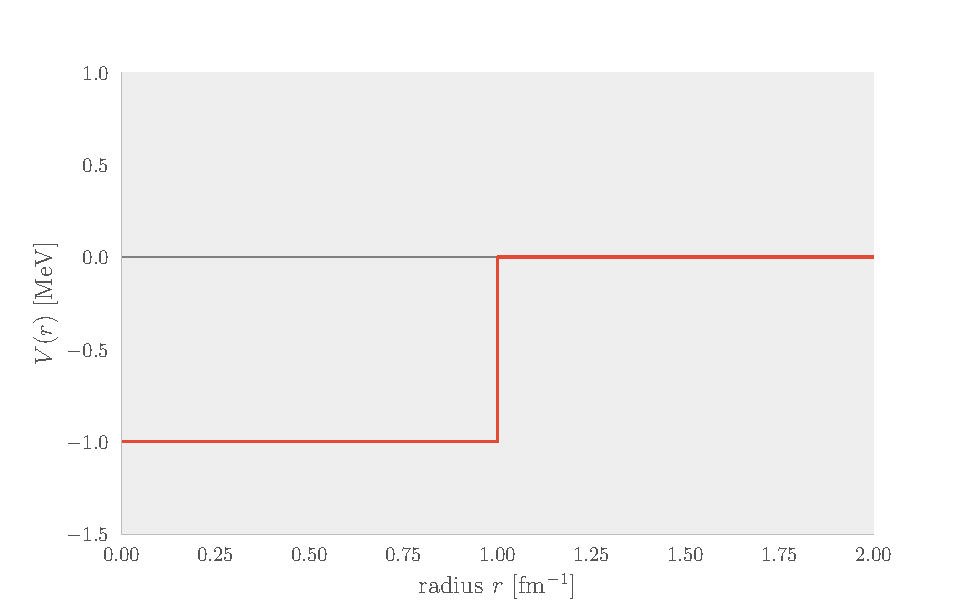
\includegraphics[]{Figures/squarewell.pdf}
  \caption{\label{fig:squarewell} An attractive square well potential with
    \(V_{0}=-1\) MeV.}
\end{figure}

[Analytical Solutions]


\subsubsection{The Yukawa Potential}
[HISTORY]

The Yukawa potential was later generalized into a class of \textit{generalized
  Yukawa potentials}. They are potentials build on superpositions of Yukawa potentials:
\begin{equation*}
  V(r) = \sum_{i=1}^{N}C_{i}\frac{e^{-\eta_{i}r}}{r}
\end{equation*}
for some coefficients \(C_{i}\) and \(\eta_{i}\).

A specific instance of a generalized Yukawa potential is the \textit{Reid
  potential}\cite{reid}. It was an incremental improvement on already existing potentials
at that time, building a parameterized potential where the exponent in each term reflects some
phenomenological properties of the nuclear force while the constants are fit to
phase shift data without consideration for their physical interpretation.
In the case of proton-neutron scattering, the potential for the partial wave
\(^{1}S_{0}\) consists of the three terms:
\begin{equation*}
  V(r) = V_{a}\frac{e^{-ax}}{x} + V_{b}\frac{e^{-bx}}{x} + V_{c}\frac{e^{-cx}}{x}
\end{equation*}
where \(x=\mu r\), \(\mu=0.7\) MeV, \(V_{a}=-10.463\) MeV, \(V_{b}=-1650.6\)
MeV, \(V_{c}=6484.3\) MeV, and \(a=1\), \(b=4\) and \(c=7\).

The individual terms are plotted in~\cref{fig:reid} along with their sum. Its
construction becomes apparent, where the three terms interact to form its three
main features: it is a short range potential, quickly falling off to zero with a
range , with
an attractive region followed by a strongly repulsive region.

\begin{figure}[ht]
  \centering
  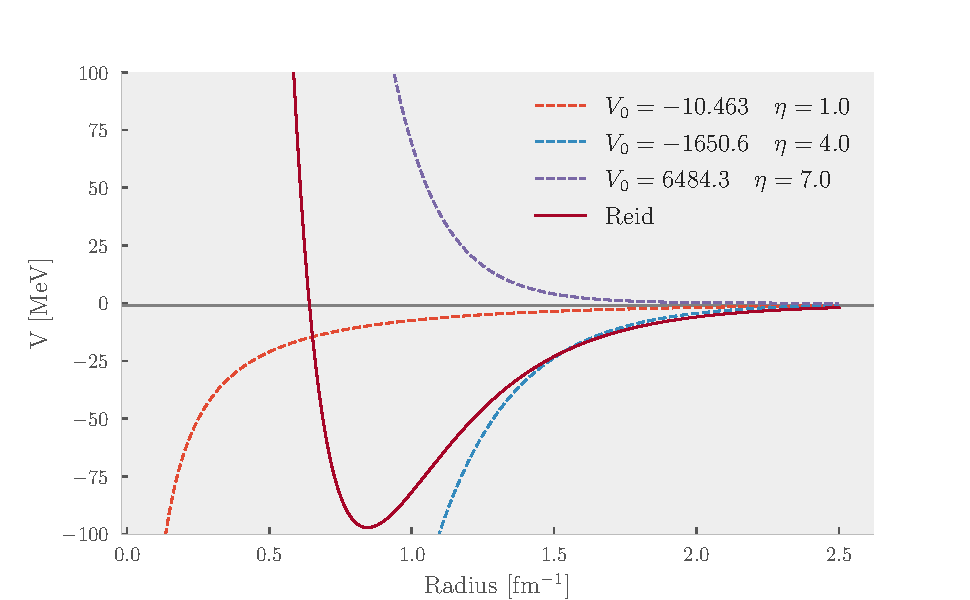
\includegraphics[]{Figures/reid.pdf}
  \caption{\label{fig:reid} The Reid potential (full stroke), a sum of three Yukawa potentials
  (dashed). It is has the typical characteristics of a nuclear force model, with
  a short range attractive potential followed by a repulsive core.}
\end{figure}

The Reid potential for \(np\) \(^{1}S_{0}\) was fit to two thousand data points
for the phase shift in the region \(0-350\) MeV, and thus should provide a good
fit in this region.

\subsubsection{Momentum Basis}

Going from position basis to momentum space requires a change of basis, achieved
through a Fourier transform. The problem is multidimensional, requiring a
generalized Fourier transform. As we are only dealing with spherically symmetric
and central potentials, the more suitable Hankel transform\footnote{The Hankel
  transform can be regarded as the Fourier transform in hyperspherical coordinates, expanding the function in
Bessel functions instead of sines and cosines. } can be used. For
\(s\)-waves, it takes the form:

\newcommand{\kp}{k^{\prime}}
\begin{align*}
  V(k, \kp{}) &= \int_{0}^{\infty}j_{0}(kr)V(r)j_{0}(k^{\prime}r)r^{2}\dd r\\
  &=  \int_{0}^{\infty}\sin(kr)V(r)\sin(k^{\prime}r)r^{2}\dd r
\end{align*}
with the notation \(V(k, \kp{}) = \mel{\kp{}}{V}{k}\). The Yukawa potential in
momentum basis is therefore
\begin{align*}
  V(k, \kp{}) &= V_{\eta} \int_{0}^{\infty}j_{0}(kr)\frac{\exp(-\eta x)}{x}j_{0}(k^{\prime}r)r^{2}\dd r\\
              &= \frac{V_{\eta}}{2\mu k\kp{}} \int_{0}^{\infty}\dd x \left( \cos{\alpha x}-\cos{\beta x} \right)\frac{\exp(-\eta x)}{x}\\
  \end{align*}
 with \(\alpha=\frac{1}{\mu}\left( k-k^{\prime} \right)\) and \(\beta =
 \frac{1}{\mu}\left( k-k^{\prime} \right)\). Adding and subtracting 1 lets us
 write the integral as

\begin{align*}
  V(k, \kp{}) &= \frac{V_{\eta}}{2\mu k\kp{}} \left[ \int_{0}^{\infty}\dd x \left( 1-\cos{\beta x} \right)\frac{\exp(-\eta x)}{x}
                - \int_{0}^{\infty}\dd x \left(1-\cos\alpha x\right) \frac{\exp(-\eta x)}{x}\right]
\end{align*}
Using a table of integrals we obtain our desired solution
\begin{align*}
  V(k, \kp{}) = \frac{V_{\eta}}{\mu k \kp{}} \ln \frac{(\mu\eta)^{2}+(k+k^{\prime})^{2}}{(\mu\eta)^{2}+(k-k^{\prime})^{2}}
\end{align*}

The Reid potential in momentum basis is simply a sum of its terms in momentum basis.




%%% Local Variables:
%%% mode: latex
%%% TeX-master: "../main"
%%% TeX-engine: xetex
%%% End:
